\documentclass[../main.tex]{subfiles}
\usepackage{fancyhdr}
\graphicspath{{../images/}}

\begin{document}
\pagestyle{fancy}
\lhead{Physics 472: Li Yang}
\chead{Homework 3}
\rhead{Junseo Shin}

\renewcommand\thefigure{\arabic{figure}} 

\paragraph*{Problem 1.} (a)
From Kittel, for a periodic delta-function potential we get the simplified equation
\begin{align*}
    \frac{P}{Ka} \sin(Ka) + \cos(Ka) = \cos(ka)
\end{align*}
where $\cos(ka) = 1$ at $k = 0$. Taking the Taylor series approximations for small $Ka$:
\begin{align*}
    \sin(Ka) &= Ka \dots \\
    \cos(Ka) &= 1 - \frac{1}{2} (Ka)^2 + \dots
\end{align*}
but if we approximate only to the first order, we get
\begin{align*}
    \frac{P}{Ka} Ka + 1 = 1 \implies P = 0
\end{align*}
which doesn't tell us any information to find the band gap
\begin{align*}
    \epsilon = \frac{\hbar^2 K^2}{2m}
\end{align*}
so we take the second order approximation for the cosine term:
\begin{align*}
    \frac{P}{Ka} Ka + 1 - \frac{1}{2} (Ka)^2 = 1 \\
    \implies K^2 = \frac{2P}{a^2}
\end{align*}
so the band gap is
\begin{align*}
    \epsilon \approx \frac{\hbar^2 P}{ma^2}
\end{align*}
(b) For $k = \pi/a$, $\cos{ka} = -1$ and the equation becomes
\begin{align*}
    \frac{P}{Ka} \sin(Ka) + \cos(Ka) = -1
\end{align*}
and from Figure \ref{hw3_1} we can approximate the Taylor series around $Ka = \pi + h$:
\begin{align*}
    f(x + h) &\approx f(x) + h f'(x) + \frac{1}{2} h^2 f''(x)
\end{align*} 
\begin{figure*}[ht]
    \centering
    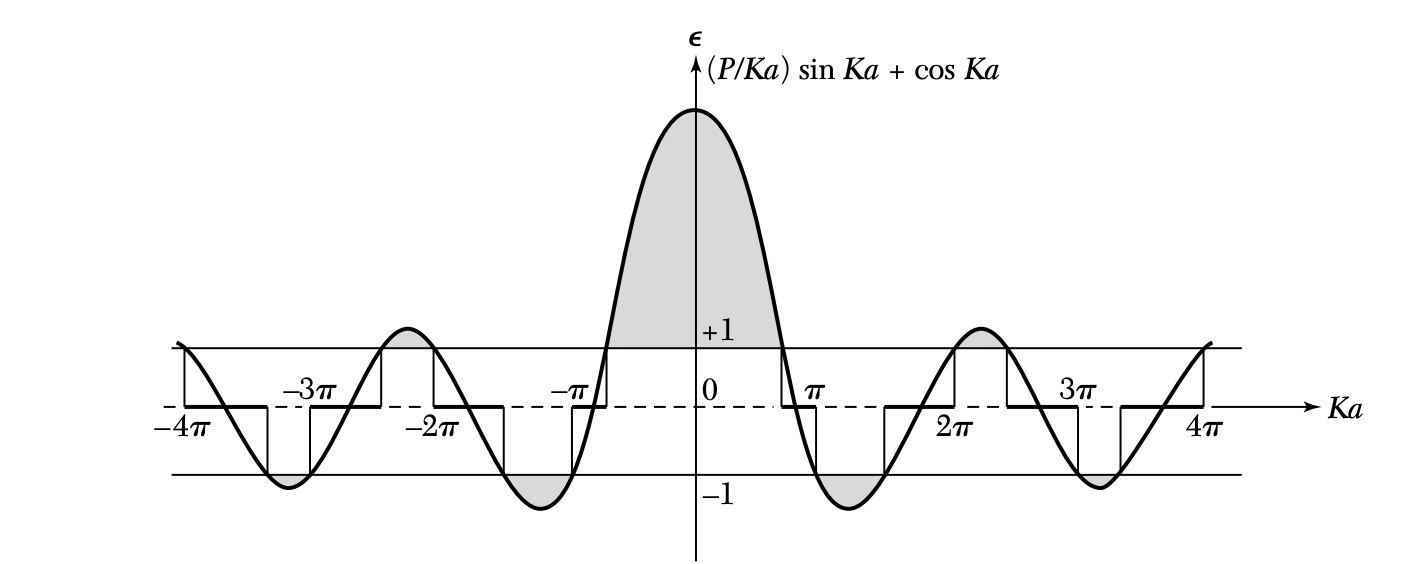
\includegraphics[width=0.7\textwidth]{hw3_1.png}
    \caption{From Kittel}
    \label{hw3_1}
\end{figure*}

so we have
\begin{align*}
    \sin(Ka) &\approx \sin \pi + h \cos{\pi} = -h \\
    \cos(Ka) &\approx \cos \pi + h (-\sin \pi) + \frac{1}{2} h^2 (-\cos \pi) = -1 + \frac{1}{2} h^2
\end{align*}
and thus
\begin{align*}
    \frac{P}{\pi} (-h) + \qt(-1 + \frac{1}{2} h^2) = -1 \\
    \implies h = \frac{2P}{\pi}
\end{align*}
where 
\begin{align*}
    (Ka)^2 = (\pi + h)^2 = \pi^2 + 2\pi h + h^2 \\
    \implies K^2 = \frac{\pi^2 + 2\pi h}{a^2} = \frac{\pi^2 + 4P}{a^2}
\end{align*}
so the band gap is 
\begin{align*}
    \epsilon \approx \frac{\hbar^2 K^2}{2ma^2}
    = \frac{\hbar^2}{2ma^2} \frac{\pi^2 + 4P}{a^2} 
\end{align*}

\paragraph*{Problem 2} Using the central equation
\begin{align*}
    (\lambda_k - \epsilon) C(k) + \sum_G U_G C(k - G) = 0
\end{align*}
where the energy gap occurs at
\begin{align*}
    k = \pm \frac{\pi}{a} \vu x + \pm \frac{\pi}{a} \vu y
\end{align*}
and from the Bragg condition $(\vb k + \vb G)^2 = k^2$ the reciprocal lattice vector is
\begin{align*}
    G = \frac{2\pi}{a} \vu x + \frac{2\pi}{a} \vu y
\end{align*}
using the relation $k - G = -\frac{\pi}{a}$ we have two equations to solve for the energy gap:
\begin{align*}
    (\lambda - \epsilon) C\qt(\frac{\pi}{a}, \frac{\pi}{a}) + U_G C\qt(-\frac{\pi}{a}, -\frac{\pi}{a}) = 0 \\
    (\lambda - \epsilon) C\qt(-\frac{\pi}{a}, -\frac{\pi}{a}) + U_G C\qt(\frac{\pi}{a}, \frac{\pi}{a}) = 0
\end{align*}
which can be written as a matrix equation
\begin{align*}
    \begin{pmatrix}
        \lambda - \epsilon & U_G \\
        U_G & \lambda - \epsilon
    \end{pmatrix}
    \begin{pmatrix}
        C\qt(\frac{\pi}{a}, \frac{\pi}{a}) \\
        C\qt(-\frac{\pi}{a}, -\frac{\pi}{a})
    \end{pmatrix}
    &= 0
\end{align*}
so the determinant of the matrix is
\begin{align*}
    (\lambda - \epsilon)^2 - U_G^2 = 0 \\
    \implies \epsilon = \lambda \pm U_G
\end{align*}
and thus the two roots tells us that the energy gap is $E_g = 2\abs{U_G}$. From the Fourier transform of the potential:
\begin{align*}
    U &= \sum_G U_G e^{i\vb G \cdot \vb r} \\
    U(x,y) &= \sum_G U_G \cos(G_x x) \cos(G_y y)
\end{align*}
so the fourier coefficients of the potential is 
\begin{align*}
    U_G &= \iint_0^a U(x,y) \cos(G_x x) \cos(G_y y) \dd{x} \dd{y} \\
    &= \iint_0^a U(x,y) \cos\qt(\frac{2\pi x}{a}) \cos\qt(\frac{2\pi y}{a}) \dd{x} \dd{y} \\
    &= 4U \frac{4}{a^2}\iint_0^a \cos^2\qt(\frac{2\pi x}{a}) \cos^2\qt(\frac{2\pi y}{a}) \dd{x} \dd{y} \\
\end{align*}
where \begin{align*}
    \int_0^a \cos^2\qt(\frac{2\pi x}{a}) \dd{x} = \frac{a}{2}
\end{align*}
so
\begin{align*}
    U_G &= -4U \frac{4}{a^2} \qt(\frac{a}{2}\frac{a}{2}) = -4U
\end{align*}
and the magnitude of the band gap is
\begin{align*}
    E_g = 2\abs{U_G} = 8U
\end{align*}
\end{document}